\documentclass{beamer}

\usetheme{metropolis}
\usepackage{natbib}
\usepackage{ulem}
\usepackage{amsmath}
\usepackage{amsthm}
\usepackage{amsfonts}
\usepackage{bm}
\usepackage{mathtools}
\usepackage{ifthen}

\newtheorem{proposition}{Proposition}
\newtheorem{assumption}{Assumption}

\theoremstyle{remark}
\newtheorem*{remark}{Remark}

\setbeamercolor{background canvas}{bg=white}

\setbeamercolor{normal text}{fg=black}
\setbeamercolor{frametitle}{bg=black, fg=white}

%%%%% macros -----------------------------------------------------------------------------

\renewcommand{\c}{\bm c}
\newcommand{\x}{\bm x}
\newcommand{\C}{\bm C}
\newcommand{\X}{\bm X}
\newcommand{\Z}{\bm Z}
\newcommand{\W}{\bm W}
\newcommand{\Xhat}{\widehat{\X}}
\newcommand \R {\mathbb{R}}

% RDPG stuff

\renewcommand{\S}{\widehat{\bm S}}
\newcommand{\U}{\widehat{\bm U}}
\newcommand{\Spop}{\bm S}
\newcommand{\Upop}{\bm U}

% mediator regression coefficients

\newcommand{\thetazero}{\bm \theta_0}
\newcommand{\thetat}{\bm \theta_\text{t}}
\newcommand{\Thetac}{\bm \Theta_\text{c}}
\newcommand{\Thetatc}{\bm \Theta_\text{tc}}

% mediator regression estimators

\newcommand \thetazerohat [1] {\widehat{\bm \theta}_0 \paren*{#1}}
\newcommand \thetathat [1] {\widehat{\bm \theta}_\text{t} \paren*{#1}}
\newcommand \Thetachat [1] {\widehat{\bm \Theta}_\text{c} \paren*{#1}}
\newcommand \Thetatchat [1] {\widehat{\bm \Theta}_\text{tc} \paren*{#1}}

% outcome regression coefficients

\newcommand{\betazero}{\beta_0}
\newcommand{\betat}{\beta_\text{t}}
\newcommand{\betac}{\beta_\text{c}}
\newcommand{\betax}{\beta_\text{x}}

% outcome regression estimators

\newcommand \betazerohat [1] {\widehat{\beta}_0 \paren*{#1}}
\newcommand \betathat [1] {\widehat{\beta}_\text{t} \paren*{#1}}
\newcommand \betachat [1] {\widehat{\beta}_\text{c} \paren*{#1}}
\newcommand \betaxhat [1] {\widehat{\beta}_\text{x} \paren*{#1}}

\newcommand \xihat [1] {\widehat{\xi} \paren*{#1}}

% causal estimands

\newcommand{\ate}{\Psi_\text{ate} \paren*{t, t^*}}
\newcommand{\cde}{\Psi_\text{cde} \paren*{t, t^*, \x}}
\newcommand{\nde}{\Psi_\text{nde} \paren*{t, t^*}}
\newcommand{\nie}{\Psi_\text{nie} \paren*{t, t^*}}

\newcommand \cdehat [1] {\widehat{\Psi}_\text{cde} \paren*{#1}}
\newcommand \ndehat [1] {\widehat{\Psi}_\text{nde} \paren*{#1}}
\newcommand \niehat [1] {\widehat{\Psi}_\text{nie} \paren*{#1}}

\newcommand{\RDPG}{\operatorname{RDPG}}
\newcommand \cond {\mid}
\newcommand \dist {\sim}

\DeclarePairedDelimiter{\paren}{(}{)}
\DeclarePairedDelimiter{\set}{\{}{\}}
\DeclarePairedDelimiter{\brac}{[}{]}
\DeclarePairedDelimiter{\norm}{\lVert}{\rVert}

\newcommand{\dx}[1][]{%
   \ifthenelse{ \equal{#1}{} }
      {\ensuremath{\;\mathrm{d}x}}
      {\ensuremath{\;\mathrm{d}#1}}
}


\renewcommand{\P}[2][]{%
   \ifthenelse{ \equal{#1}{} }
      {\ensuremath{\mathbb{P} \brac*{#2}}}
      {\ensuremath{\mathbb{P} \brac*{#2 \mid #1}}}
}

\newcommand{\E}[2][]{%
   \ifthenelse{ \equal{#1}{} }
      {\ensuremath{\mathbb{E} \brac*{#2}}}
      {\ensuremath{\mathbb{E} \brac*{#2 \mid #1}}}
}

%%%%% end macros ------------------------------------------------------------------
\hypersetup{colorlinks,citecolor=cyan, urlcolor=cyan, linkcolor=black}

\title{Estimating network-mediated causal effects via spectral embeddings}
\date{2022-10-14, SGSA Seminar}
\author{Alex Hayes and Keith Levin}
\institute{University of Wisconsin-Madison}


\begin{document}

\maketitle

\begin{frame}{Setting}
    \begin{columns}
        \column{0.45\textwidth}

        \begin{figure}
            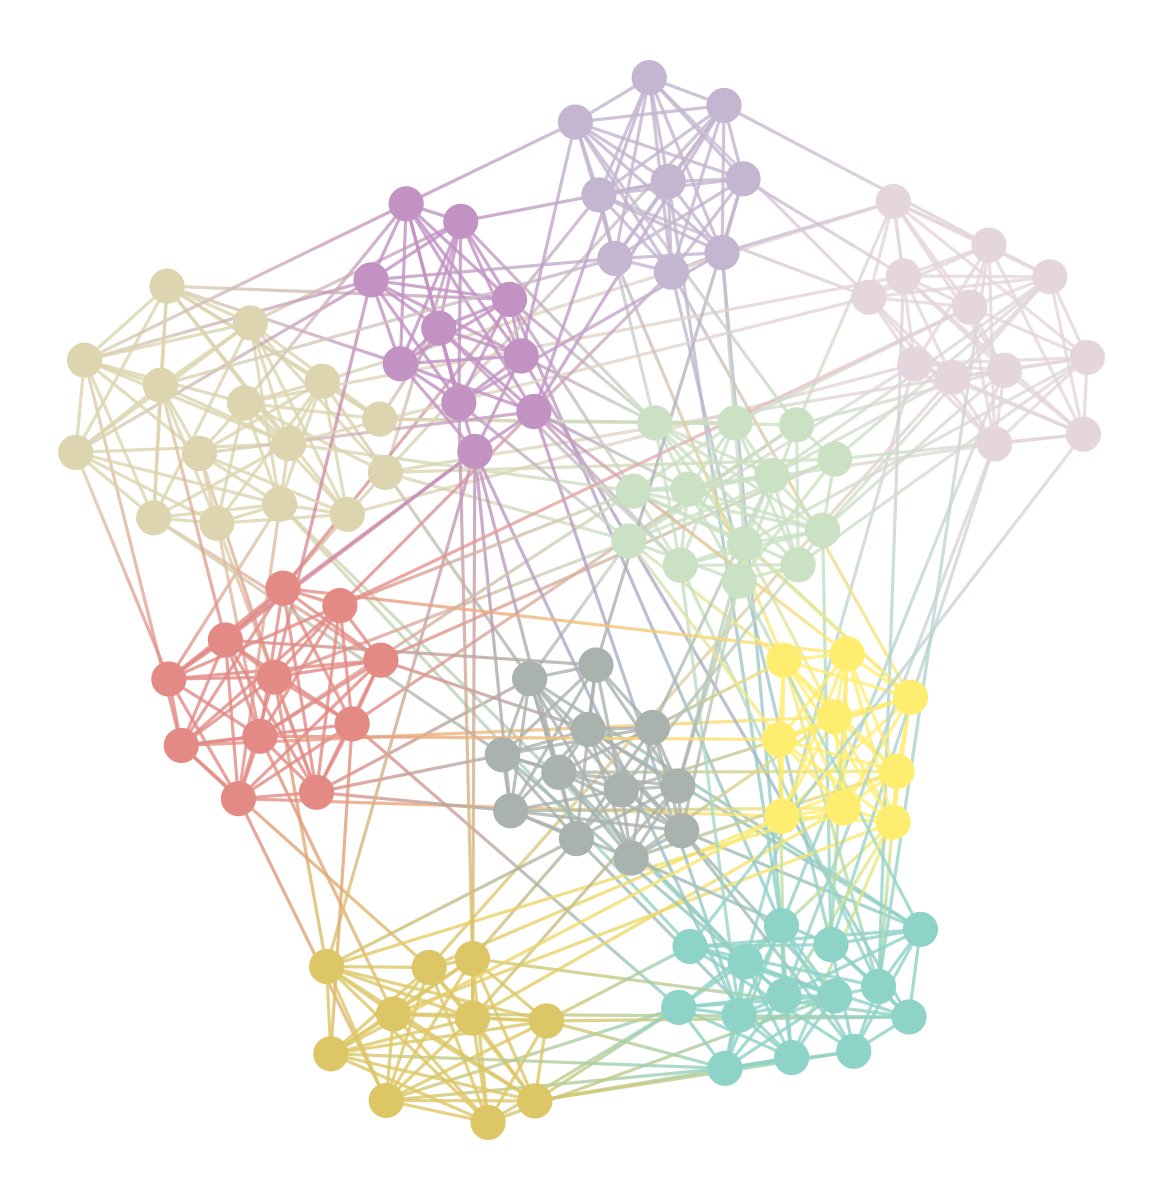
\includegraphics[width=\textwidth]{figures/assortative.png}
        \end{figure}

        \column{0.55\textwidth}

        Network $A \in \set{0, 1}^{n \times n}$

        Nodal covariates $\W_1, ..., \W_n \in \R^{p}$

        Nodal outcomes $Y_1, ..., Y_n \in \R$

    \end{columns}
\end{frame}

\begin{frame}{Network model: stochastic blockmodel (SBM)}
    \begin{columns}
        \column{0.45\textwidth}

        \begin{figure}
            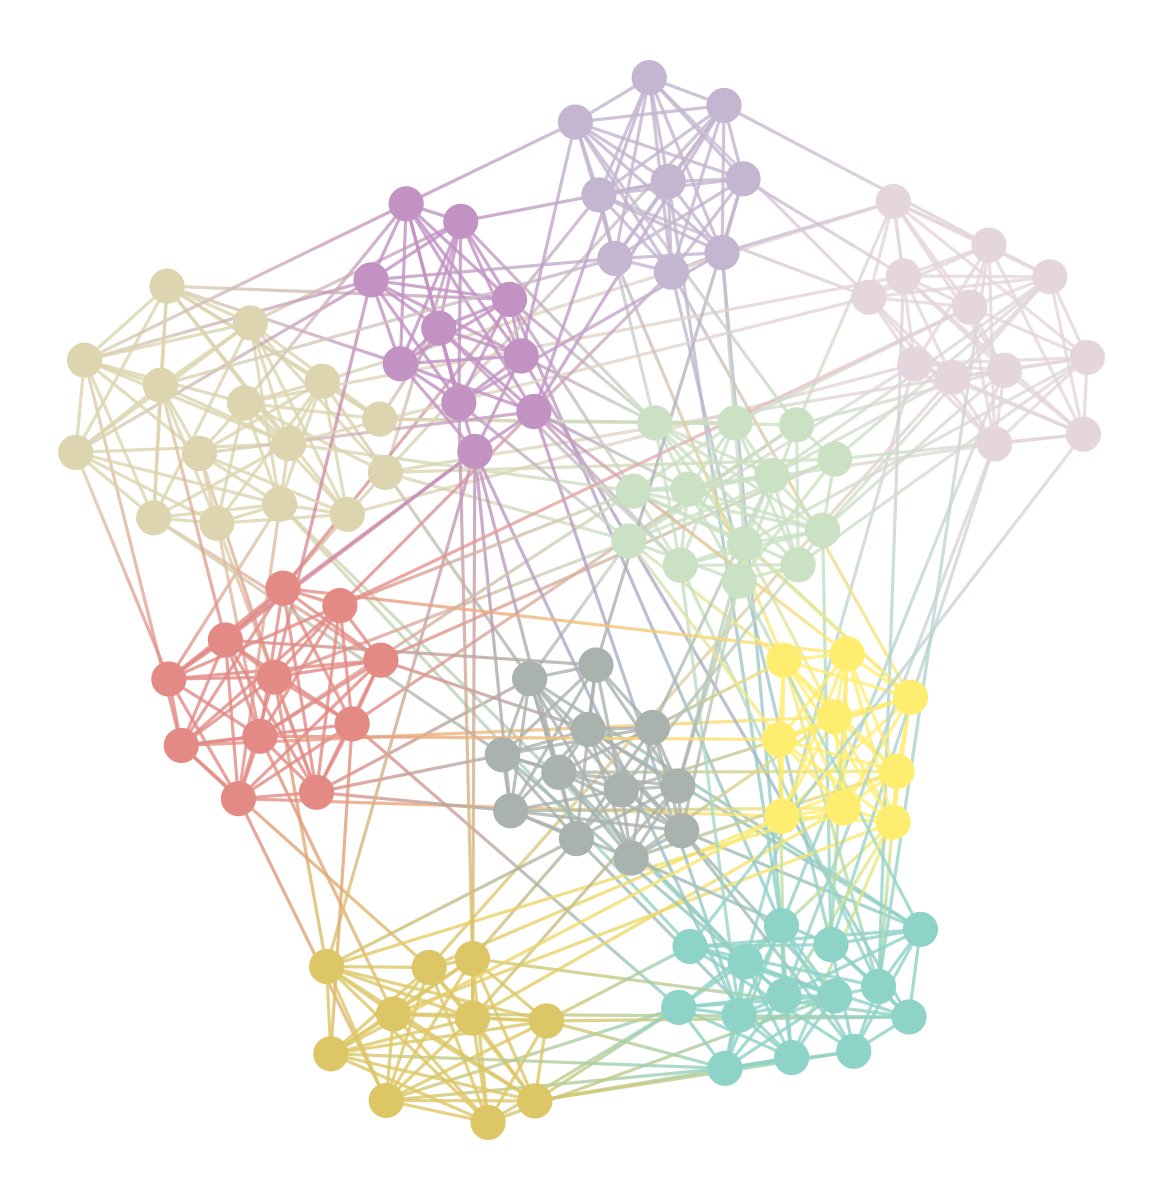
\includegraphics[width=\textwidth]{figures/assortative.png}
        \end{figure}

        \column{0.55\textwidth}

        \textbf{Degree-corrected SBM}

        \vspace{4mm}

        $k$ ``blocks'' or communities
        $\Z_i \in \set{0, 1}^k$ one-hot indicator of node $i$'s block

        \vspace{3mm}

        $\gamma_i \in [0, 1]$ node $i$'s popularity
        $B \in [0, 1]^{k \times k}$ inter-block edge probabilities

        \begin{align*}
            \P[\Z, \gamma]{A_{ij} = 1} = \gamma_i \cdot \Z_i B \Z_j^T \cdot \gamma_j
        \end{align*}

    \end{columns}
\end{frame}

\begin{frame}{Latent positions in the SBM}

    \begin{align*}
        \P[\Z, B]{A} & =
        \underbrace{
            \begin{bmatrix}
                1 & 0 \\
                1 & 0 \\
                0 & 1 \\
                0 & 1 \\
            \end{bmatrix}
        }_{\Z}
        \underbrace{
            \begin{bmatrix}
                0.6  & 0.02 \\
                0.02 & 0.6
            \end{bmatrix}
        }_{B}
        \underbrace{
            \begin{bmatrix}
                1 & 1 & 0 & 0 \\
                0 & 0 & 1 & 1 \\
            \end{bmatrix}
        }_{\Z^T}         \\
        \P[\Z, B]{A} & =
        \begin{bmatrix}
            0.6  & 0.6  & 0.02 & 0.02 \\
            0.6  & 0.6  & 0.02 & 0.02 \\
            0.02 & 0.02 & 0.6  & 0.6  \\
            0.02 & 0.02 & 0.6  & 0.6  \\
        \end{bmatrix}
    \end{align*}

\end{frame}

\begin{frame}{Intuition: incorporate latent positions into regression}

    \begin{align*}
        \underbrace{
            \begin{bmatrix}
                y_1 \\
                y_2 \\
                y_3 \\
                y_4 \\
            \end{bmatrix}
        }_\text{outcome}
         & =
        \underbrace{
            \begin{bmatrix}
                2.02  & 0.81  \\
                -0.04 & -1.83 \\
                0.76  & -0.58 \\
                -0.34 & -0.50 \\
            \end{bmatrix}
        }_{\W}
        \underbrace{
            \begin{bmatrix}
                0.3 \\
                9.6
            \end{bmatrix}
        }_{\beta_\text{w}}
        +
        \underbrace{
            \begin{bmatrix}
                1 & 0 \\
                1 & 0 \\
                0 & 1 \\
                0 & 1 \\
            \end{bmatrix}
        }_{\Z}
        \underbrace{
            \begin{bmatrix}
                0.5 \\
                0.3
            \end{bmatrix}
        }_{\beta_\text{z}}
        +
        \underbrace{
            \begin{bmatrix}
                \varepsilon_1 \\
                \varepsilon_2 \\
                \varepsilon_3 \\
                \varepsilon_4 \\
            \end{bmatrix}
        }_\text{error}
    \end{align*}

    $\beta_\text{z}$ describes impact of belonging to particular block

\end{frame}

\begin{frame}{Problem: SBMs are not very expressive network models}

    Solution: random dot product graphs

    \begin{align*}
        A_{ij} \cond \X & \dist \mathrm{Bernoulli} \paren*{\X_i^T \X_j} \\
        \X_i            & \dist F
    \end{align*}

    $F$ is a $k \ll n$ dimensional inner product distribution. Then

    \begin{align*}
        \E[\X]{A} & = \X \X^T = \Upop \Spop \Upop^T
    \end{align*}

    Define $\X = \Upop \Spop^{1/2} \in \mathbb{R}^{n \times k}$ to be the \emph{latent positions}

\end{frame}

\begin{frame}{Regression incorporating network principle components}

    Regression with rank-$k$ truncated eigendecomposition of $A$

    \begin{align*}
        \E[\X]{A}           & = \X \X^T = \Upop \Spop \Upop^T                         \\
        \E[\W_i, \X_i]{Y_i} & = \betazero + \W_i \beta_\text{w} + \X_i \beta_\text{x}
    \end{align*}

    $\beta_\text{x}$ still roughly ``effect of belonging to block $Z_i$ with popularity $\gamma_i$'', but $\beta_\text{x}$ is rotationally unidentifiable

\end{frame}

\begin{frame}{Regression incorporating network principle components}

    This has been done in \cite{le_linear_2021}!

    \begin{align*}
        \E[\W_i, A]{Y_i} & = \W_i \beta_\text{w} + \xi + \alpha
    \end{align*}

    Define $S_k$ to be truncated eigenspace of $\E[\X]{A}$ and  $\mathcal R = \mathrm{col}(\W) \cap S_k$. Require $\xi \in \mathcal R$, $\W_i \beta_\text{w} \perp \mathcal R$ and $\alpha \perp \mathcal R$

    \begin{align*}
        \E[\W_i, A]{Y_i} =
        \underbrace{\W_i \beta_\text{w}}_\text{covariate effect} +
        \underbrace{\W_i \theta}_\text{joint network covariate effect} +
        \underbrace{\alpha}_\text{network effect}
    \end{align*}

    Solves an identifiability issue we sweep under the rug
\end{frame}

\begin{frame}{AddHealth data from \cite{le_linear_2021}}

    \begin{itemize}
        \item Data on 2,152 high school students (nodes)
        \item 7,986 self-reported friendships (edges)
        \item Outcome: measure of mental health
        \item Covariates: race, sex, grade in school
    \end{itemize}

    \begin{columns}
        \column{0.5\textwidth}

        \begin{figure}
            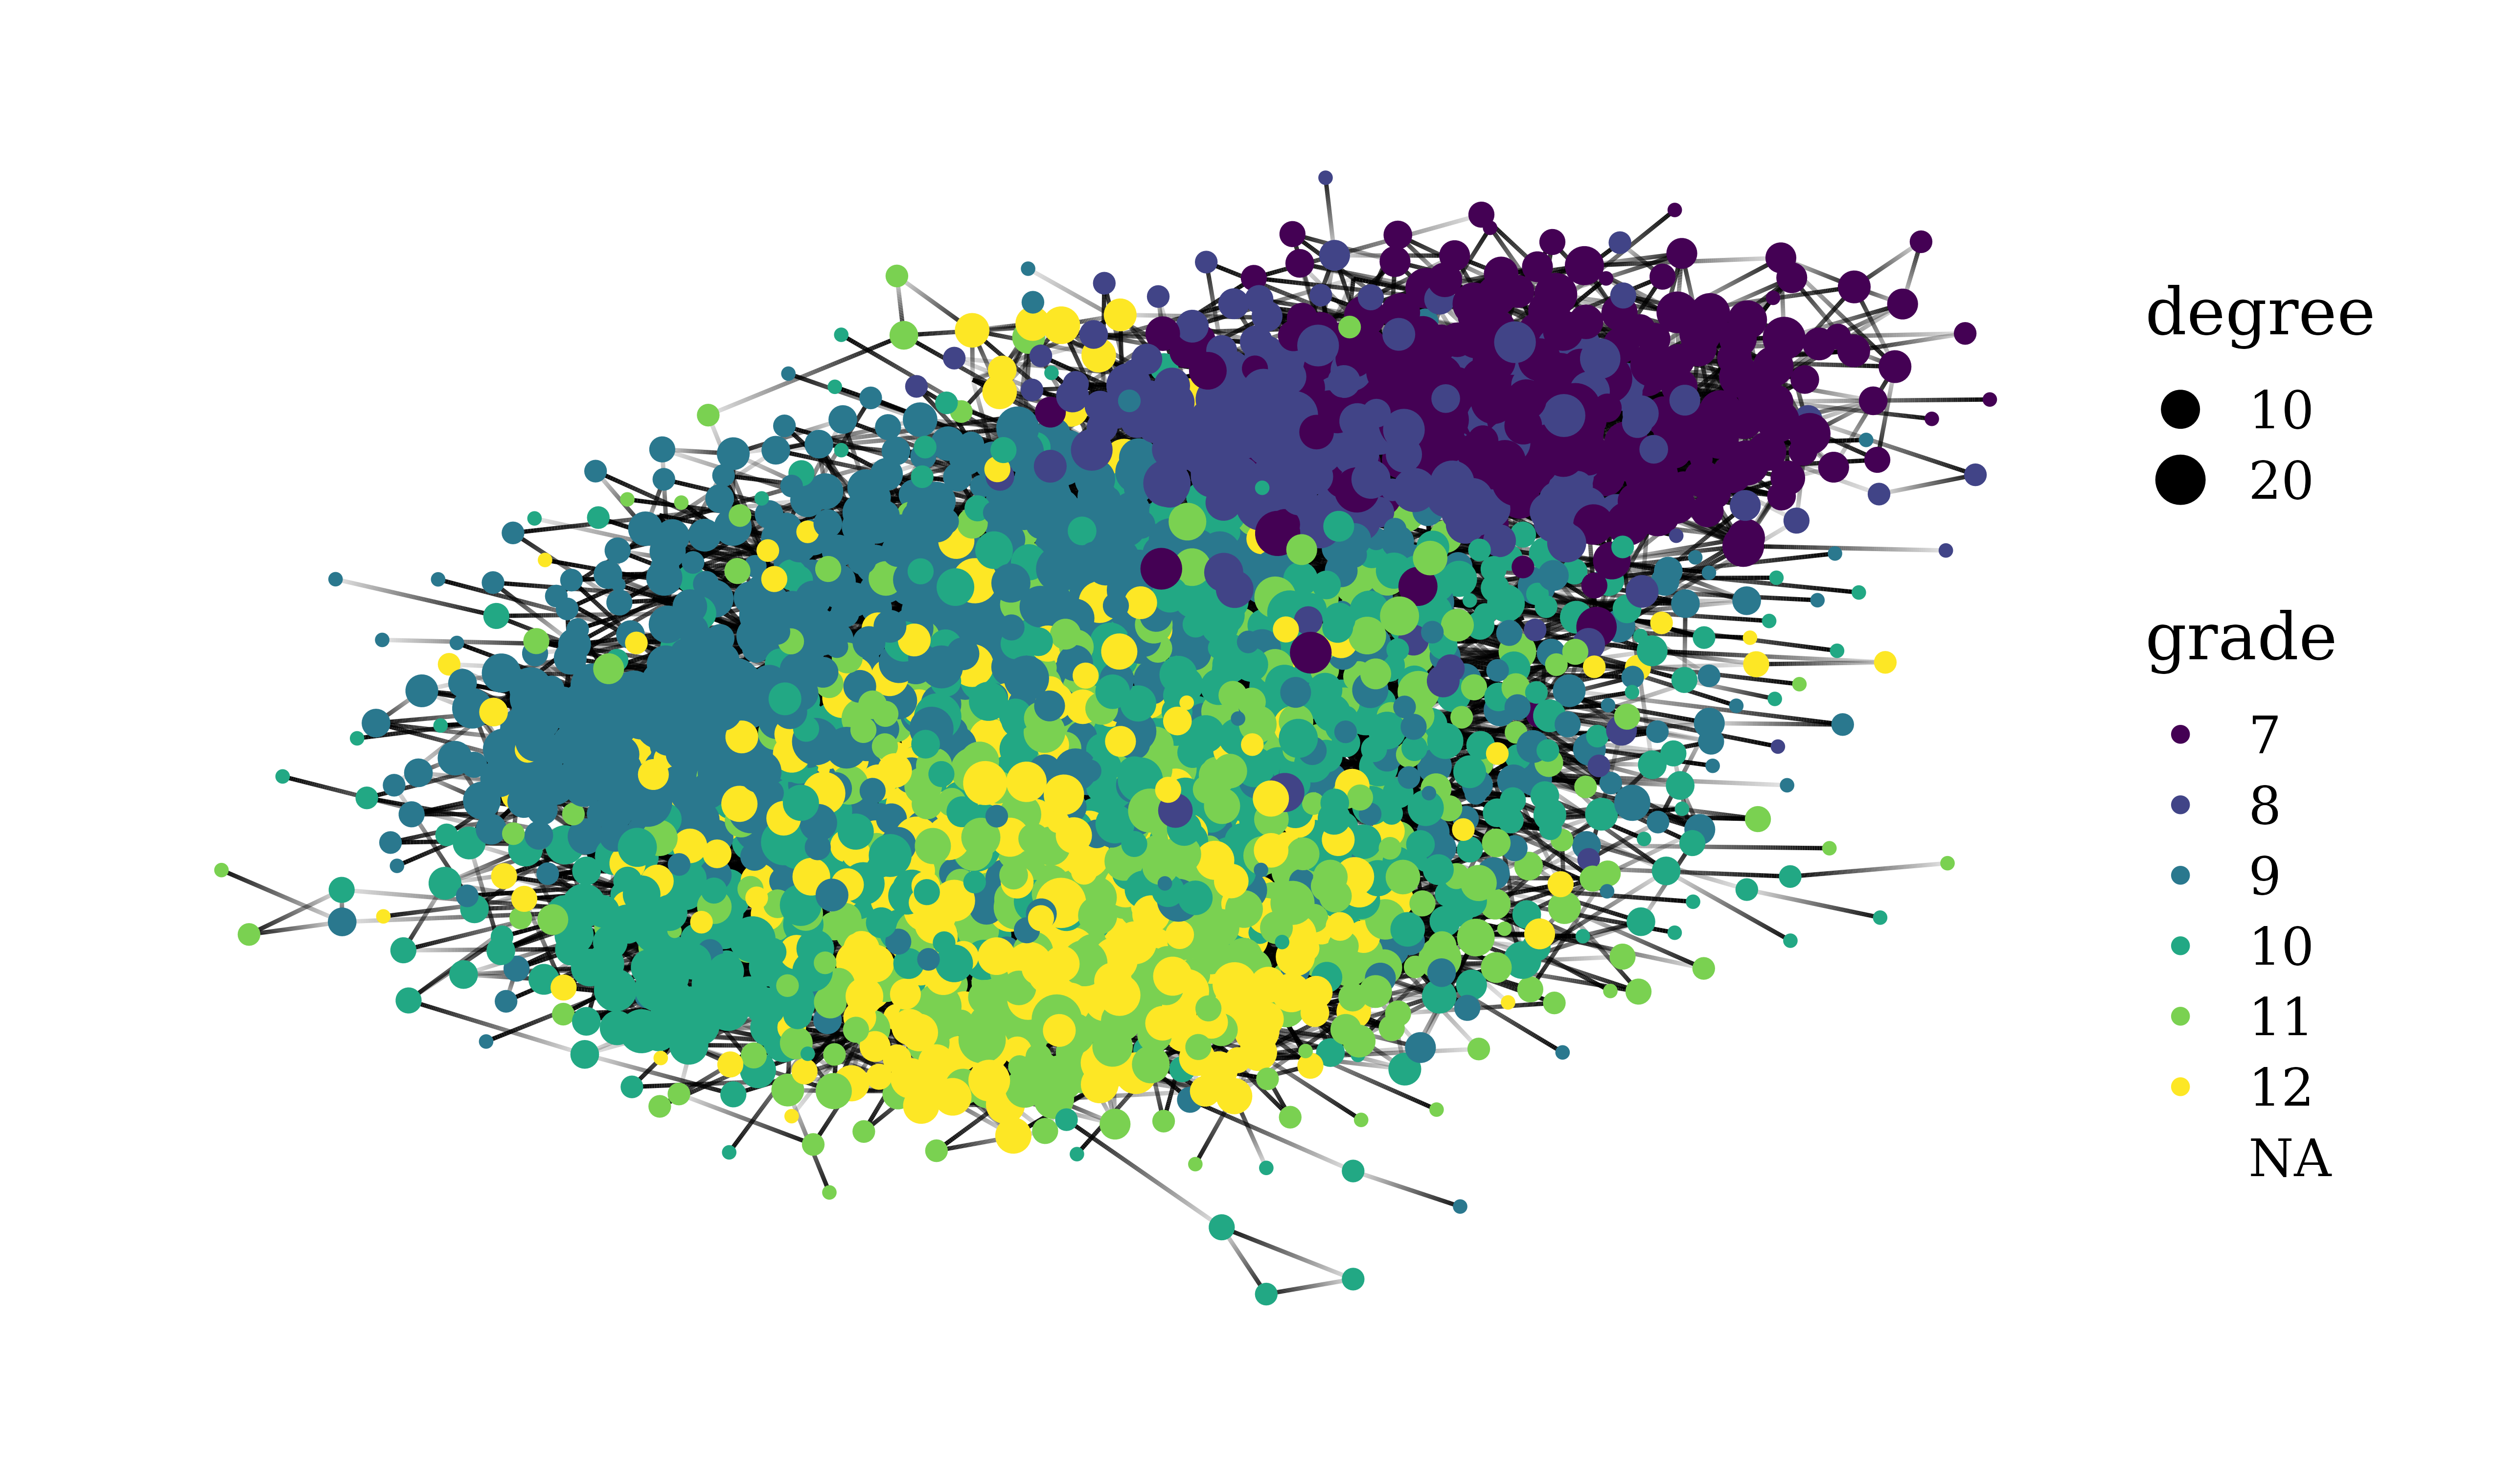
\includegraphics[width=\textwidth]{figures/presentation/homophily-grade.png}
            \caption{Grade based homophily in a high school social network.}
            \label{fig:homophily-grade}
        \end{figure}

        \column{0.5\textwidth}

        \begin{figure}
            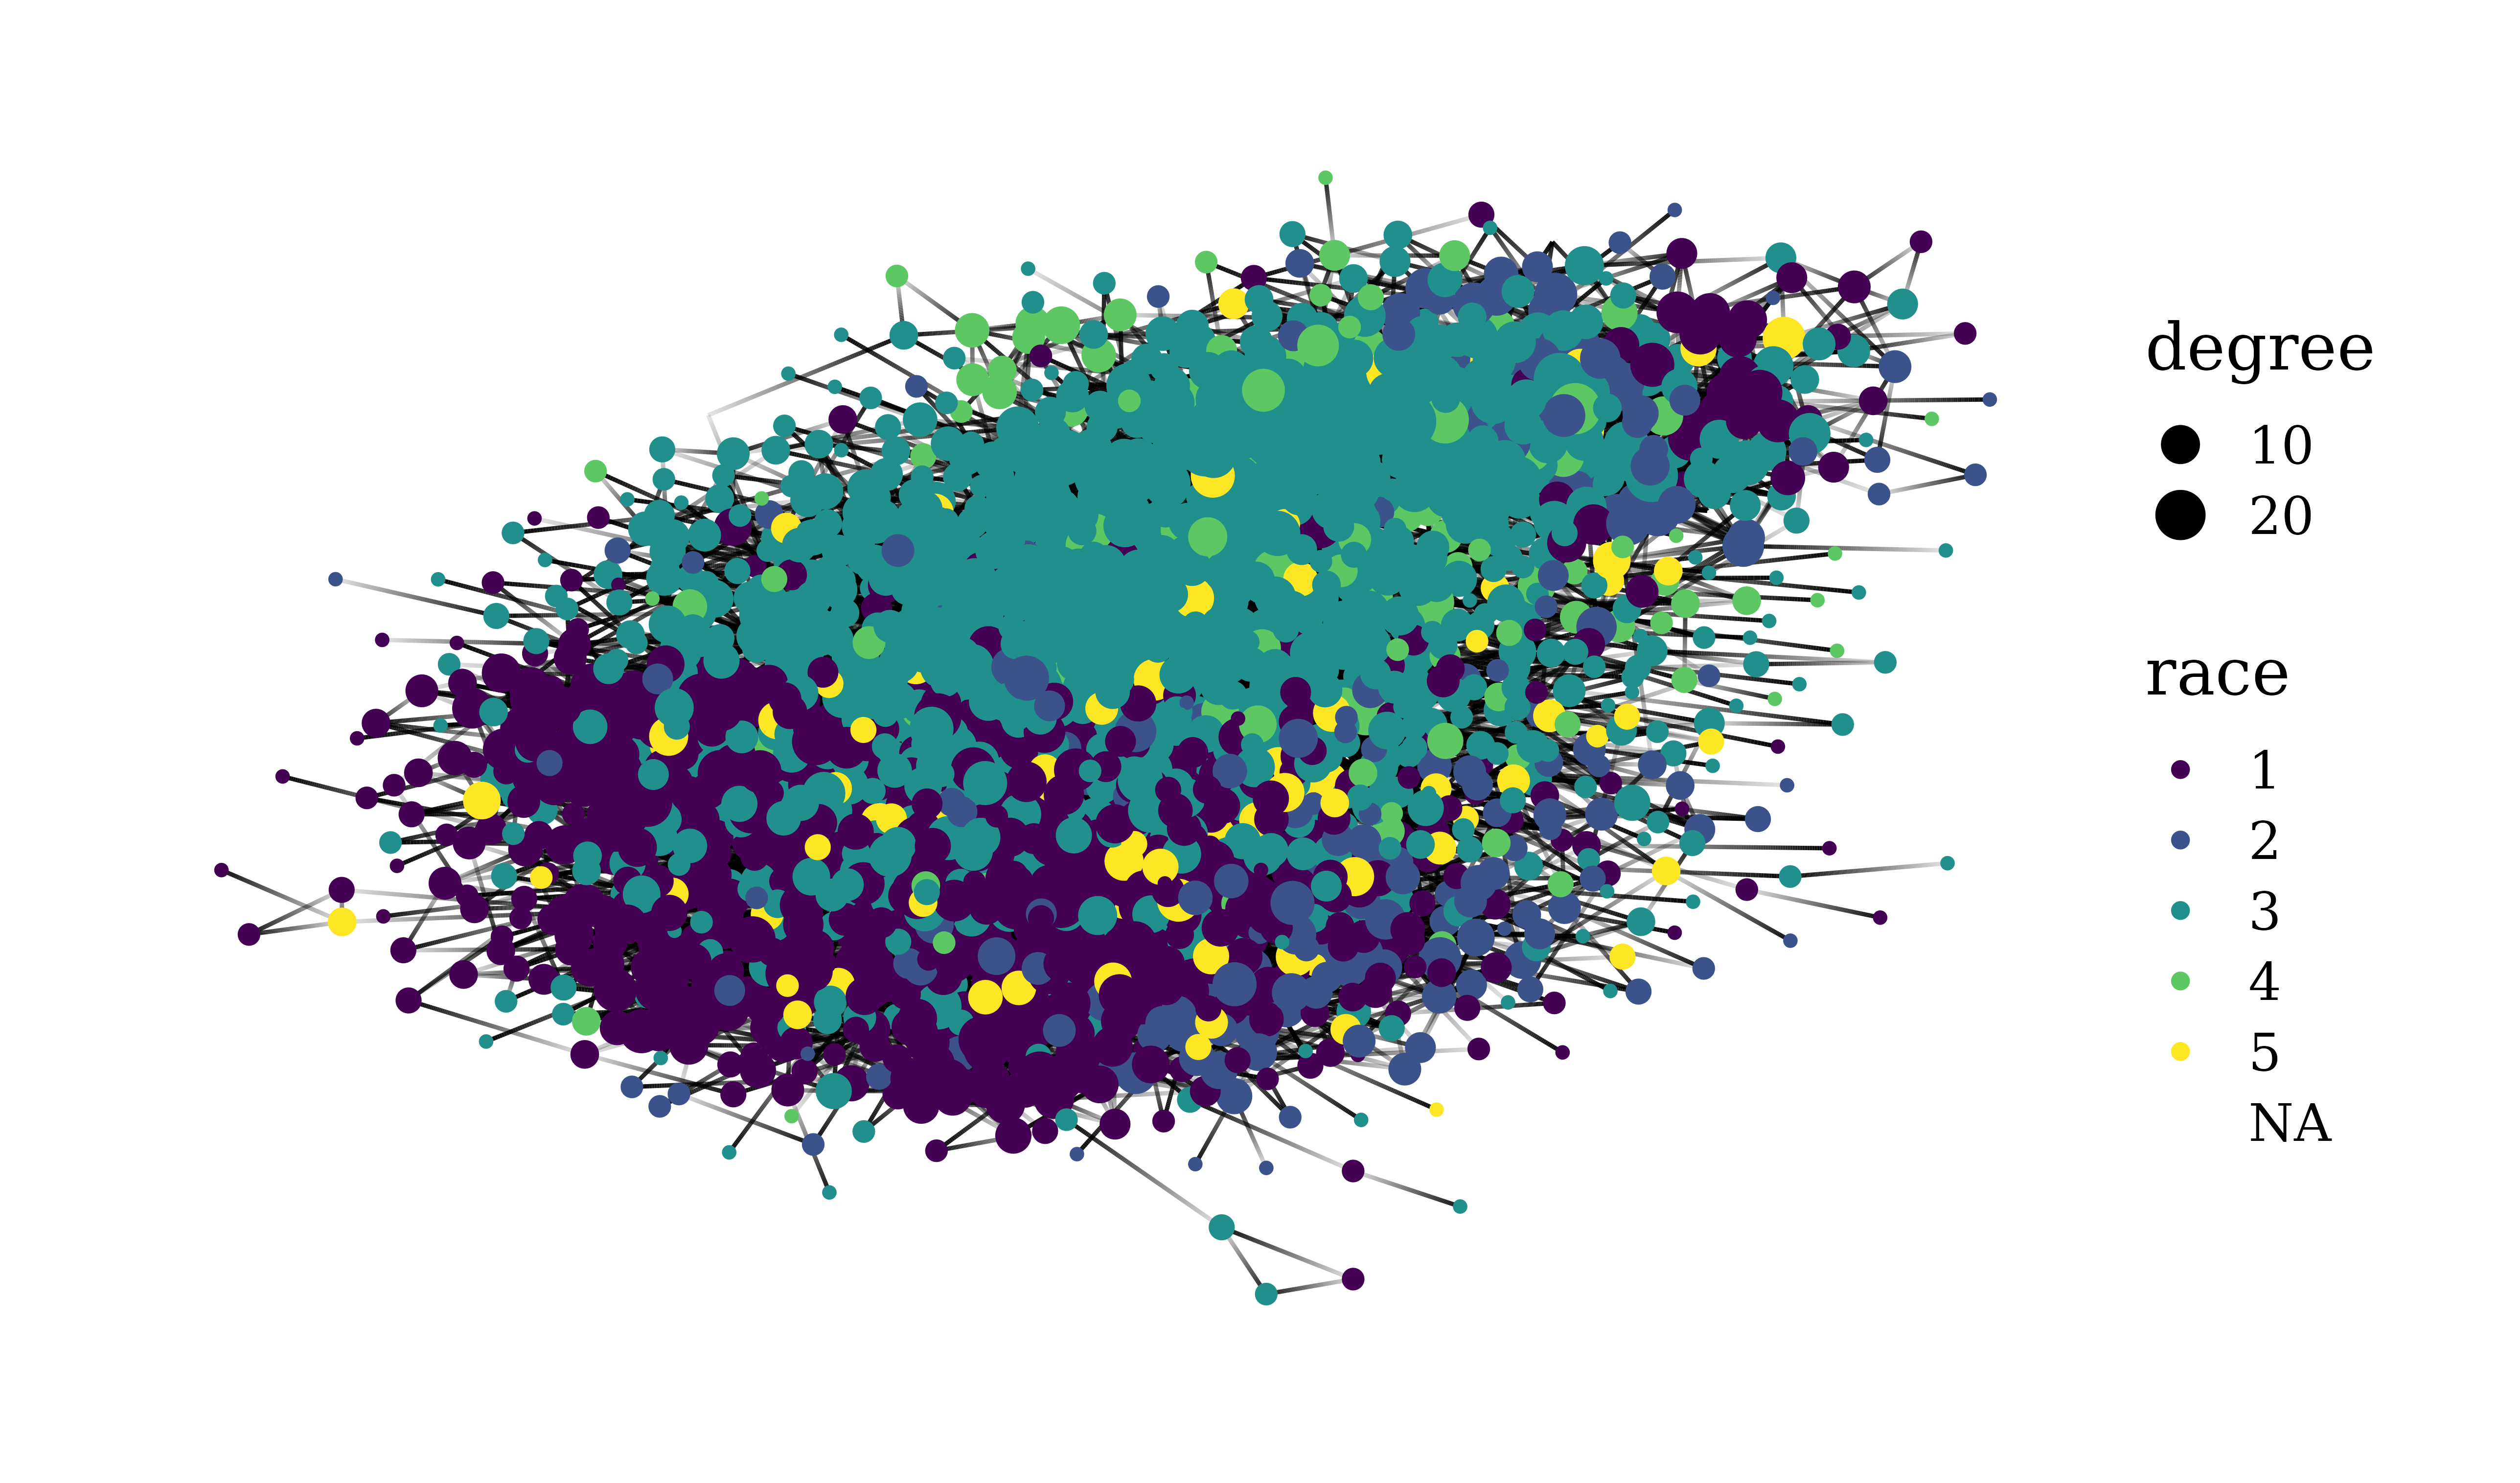
\includegraphics[width=\textwidth]{figures/presentation/homophily-race.png}
            \caption{Race based homophily in a high school social network.}
            \label{fig:homophily-race}
        \end{figure}

    \end{columns}
\end{frame}

\begin{frame}{Results when applied to AddHealth data}

    \begin{itemize}
        \item dimension $k$ of latent space estimated to be 9
        \item $\mathrm{dim}(\mathcal R)$ estimated to be zero, interpreted as no network-outcome confounding
        \item $\alpha$: strong and significant network effect
        \item $\beta_\text{w}$: significant sex and grade effects conditional on network
        \item $\beta_\text{w}$: weak effect of race conditional on network
        \item OLS estimates strong effect of race unconditional on network
    \end{itemize}

\end{frame}

\begin{frame}{Results when applied to AddHealth data: a mystery}

    \begin{itemize}
        \item dimension $k$ of latent space estimated to be 9
        \item $\mathrm{dim}(\mathcal R)$ estimated to be zero, interpreted as no network-outcome confounding
        \item $\alpha$: strong and significant network effect
        \item $\beta_\text{w}$: significant sex and grade effects conditional on network
        \item \textcolor{cyan}{$\beta_\text{w}$: weak effect of race conditional on network}
        \item \textcolor{cyan}{OLS estimates strong effect of race unconditional on network}
    \end{itemize}

    Why does controlling for latent position in network make the race coefficient go away?

\end{frame}

\begin{frame}{Spoiler}

    \begin{figure}
        \centering
        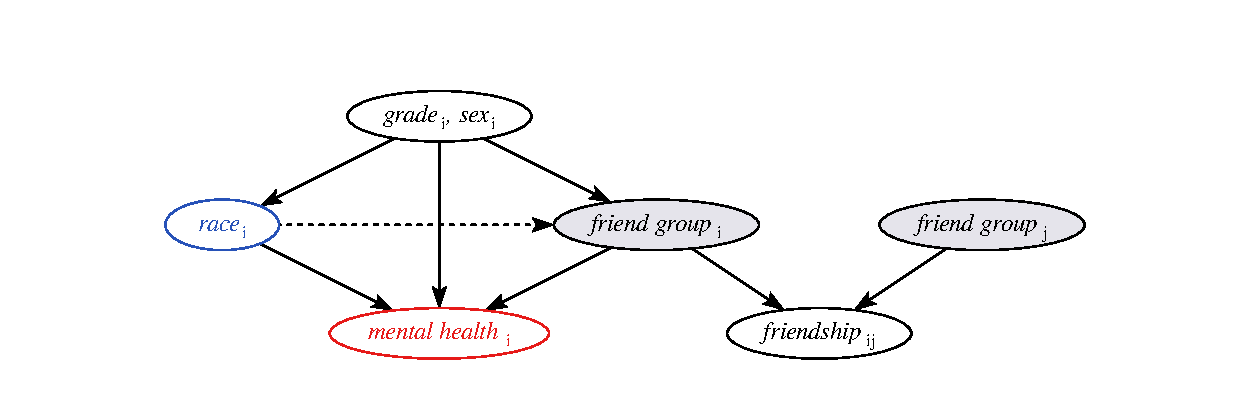
\includegraphics[width=\textwidth]{figures/addhealth-dag.pdf}
        \caption{Results are consistent with this causal model, where race causes group membership and group membership causes mental health. Controlling for friend group (position in network) leads to overcontrol bias when estimating the average treatment effect of race}
        \label{fig:addhealth-dag}
    \end{figure}

    % NOTE: grade to race arrow doesn't make any sense

\end{frame}

\begin{frame}{Causal reduced rank network regression}
    \begin{columns}
        \column{0.45\textwidth}

        \begin{figure}
            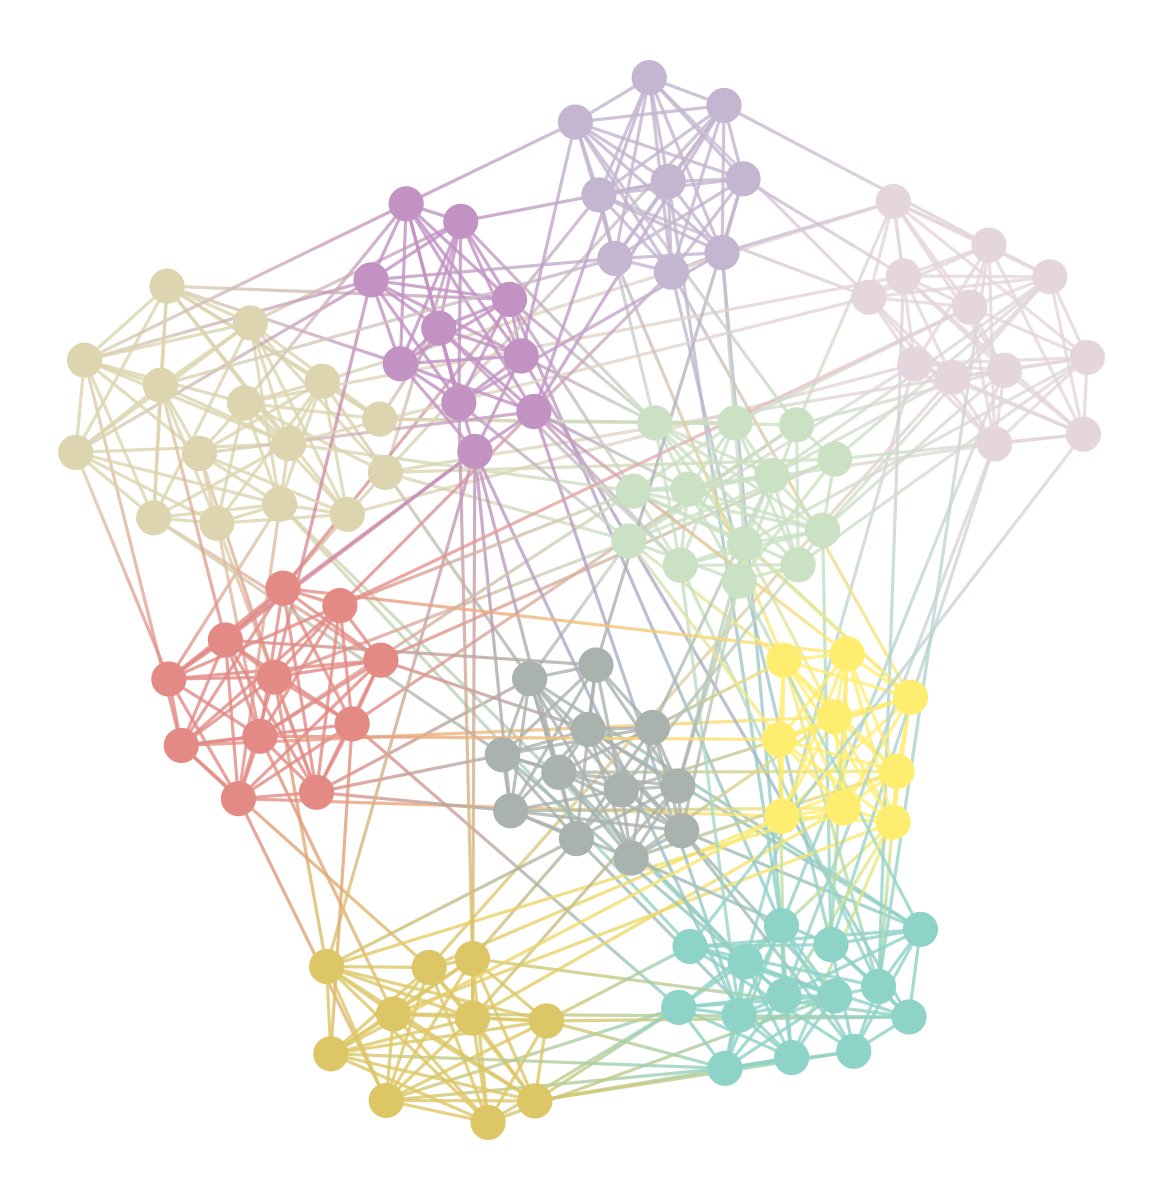
\includegraphics[width=\textwidth]{figures/assortative.png}
        \end{figure}

        \column{0.55\textwidth}

        Network $A \in \set{0, 1}^{n \times n}$

        Nodal covariates $\W_1, ..., \W_n \in \R^{p + 1}$

        Nodal outcomes $Y_1, ..., Y_n \in \R$

        \vspace{6mm}

        Partition $\W_i = (T_i, \C_i)$

        Treatment $T_i \in \set{0, 1}$

        Controls $\C_i \in \R^p$

        \vspace{6mm}

        No interference or contagion!
    \end{columns}
\end{frame}


\begin{frame}{Interpreting regression coefficients}

    \textbf{In observational settings:} $\beta_\text{t} = 2$ implies that, on average, a one-unit increase in $T_i$ is associated with a two-unit increase in $Y_i$

    \textbf{When controlling for all confounders:} $\beta_\text{t} = 2$ is an estimate of the \emph{average treatment effect}

    $\beta_\text{t}$ can also estimate \emph{other causal quantities} \citep{vanderweele_explanation_2015}

\end{frame}

\begin{frame}{Causal estimands}

    \begin{itemize}
        \item \emph{Average treatment effect}: how much the outcome $Y$ would change on average if the treatment $T$ were changed from $T = t$ to $T = t^*$

              \begin{equation*}
                  \ate = \E{Y_t - Y_{t^*}}
              \end{equation*}

              % question: is this controlling for covariates?

        \item \emph{Controlled direct effect}: how much the outcome $Y$ would change on average if the mediator $\X$ were fixed at level $\x$ uniformly in the population, but the treatment were changed from $T = t$ to $T = t^*$

              \begin{equation*}
                  \cde = \E{Y_{t \, \x} - Y_{t^* \, \x}}
              \end{equation*}

    \end{itemize}

\end{frame}

\begin{frame}{Causal estimands}

    \begin{itemize}
        \item \emph{Natural direct effect}: how much the outcome $Y$ would change if the exposure $T$ were set at level $T = t^*$ versus $T = t$ but for each individual the mediator $\X$ were kept at the level it would have taken, for that individual, if $T$ had been set to $t^*$

              \begin{equation*}
                  \nde = \E{Y_{t \, \X_{t^*}} - Y_{t^* \, \X_{t^*}}}
              \end{equation*}

        \item Captures the effect of the exposure on the outcome that would remain if we were to disable the pathway from the exposure to the mediator

    \end{itemize}

\end{frame}

\begin{frame}{Causal estimands}

    \begin{itemize}
        \item \emph{Natural indirect effect}: how much the outcome $Y$ would change on average if the exposure were fixed at level $T = t^*$ but the mediator $\X$ were changed from the level it would take if $T=t$ to the level it would take if $T = t^*$

              \begin{equation*}
                  \nie = \E{Y_{t \, \X_{t}} - Y_{t \, \X_{t^*}}}
              \end{equation*}

        \item Captures the effect of the exposure on the outcome that operates by changing the mediator
    \end{itemize}

    \begin{equation*}
        \ate = \nde + \nie
    \end{equation*}

\end{frame}

\begin{frame}{Identifying assumptions for mediated effects}

    \centering

    \begin{figure}
        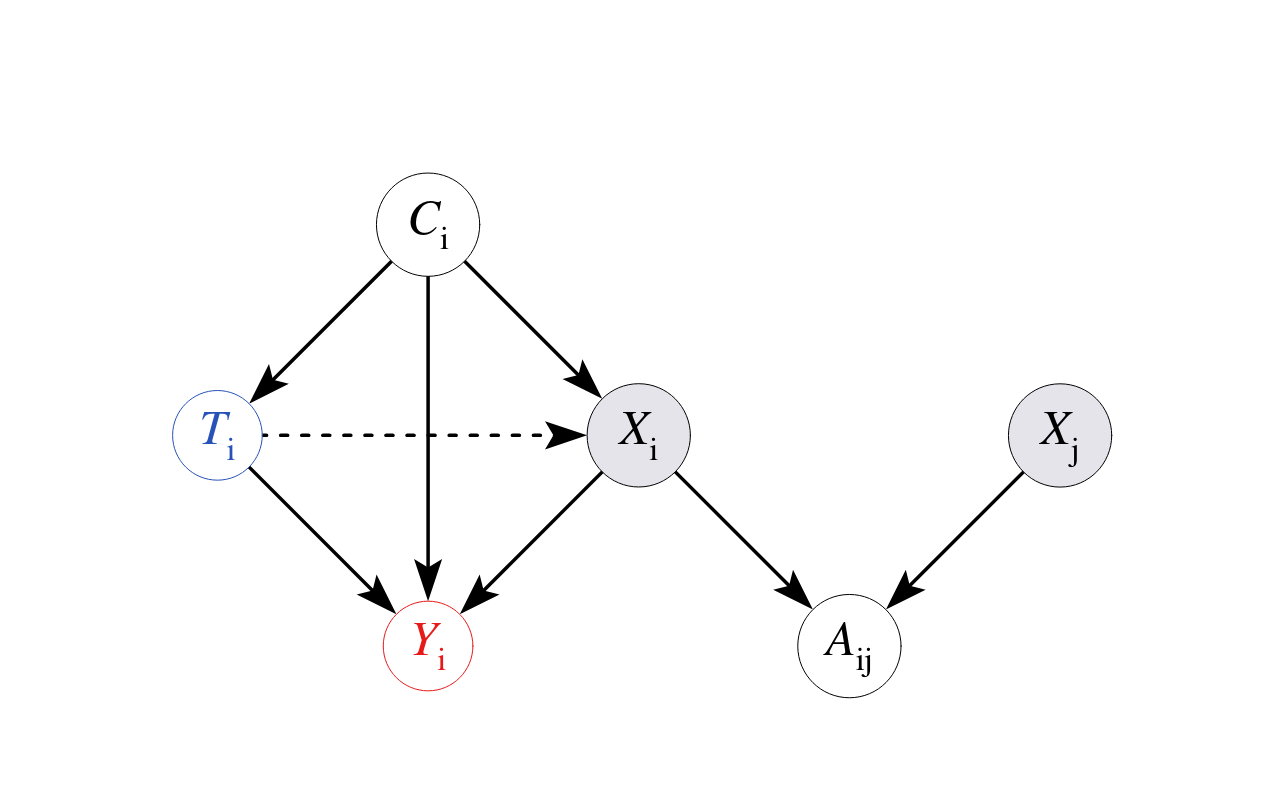
\includegraphics[width=0.9\textwidth]{figures/mediating.png}
        \caption{Directed acyclic graph (DAG) relating for node $i$ in a reduced rank network regression model. Portions of the DAG corresponding to nodes $j \neq i$ are omitted. $\X_i$ and $\X_j$ are not observed.}
        \label{fig:mediating}
    \end{figure}

\end{frame}





\begin{frame}{Consequences for regressions}

    Suppose the latent positions $\X$ are mediators. Then:

    \begin{itemize}
        \item Network regressions $\beta$ equal the \emph{natural direct effect} of $T$ on $Y$, not the average treatment effect
        \item If we compute a separate regression, we can compute the \emph{natural indirect effect} of $T$ on $Y$ (i.e. race causes group memberships causes mental health outcomes)
        \item These two effects add up to the average treatment effect
        \item Ordinary least squares ignoring the network structure can be used to estimate the \emph{average treatment effect}
    \end{itemize}

\end{frame}

\begin{frame}{A causal re-interpretation of \cite{le_linear_2021}'s results}

    Under mediation model:

    \begin{itemize}
        \item dimension $k$ of latent space estimated to be 9
        \item $\mathrm{dim}(\mathcal R)$ estimated to be zero, \sout{interpreted as no network-outcome confounding} \textcolor{cyan}{race, grade and sex do not perfectly cause membership in any friend group}
        \item $\alpha$: strong and \textcolor{cyan}{causal} effect of friend group on mental health
        \item $\beta_\text{w}$: significant sex and grade \textcolor{cyan}{natural direct effects}
        \item $\beta_\text{w}$: small \textcolor{cyan}{natural direct effect} of race
        \item OLS estimates large \textcolor{cyan}{average treatment effect} of race
    \end{itemize}

    \textcolor{cyan}{Since $\Psi_\text{ate} = \Psi_\text{nde} + \Psi_\text{nie}$ and $\Psi_\text{ate}$ is large and $\Psi_\text{nde}$ is small, $\Psi_\text{nie}$ must be large; there is large \emph{natural indirect effect} of race on mental health}

\end{frame}

\begin{frame}{Semi-parametric causal identification}

    If the mediation DAG holds (non-parametric assumption!) and additionally

    \begin{align*}
        \underbrace{\E[T, \C, \X]{Y}}_{\mathbb R}
         & = \underbrace{\betazero}_{\mathbb R}
        + \underbrace{t}_{\{0, 1\}} \underbrace{\betat}_{\mathbb R}
        + \underbrace{\c}_{\mathbb R^{1 \times p}} \underbrace{\betac}_{\mathbb R^p}
        + \underbrace{\x}_{\mathbb R^{1 \times k}} \underbrace{\betax}_{\mathbb R^k} \\
        \underbrace{\E[T, \C]{\X}}_{\mathbb R^{1 \times k}}
         & = \underbrace{\thetazero}_{\mathbb R^{1 \times k}}
        + \underbrace{t}_{\{0, 1\}} \underbrace{\thetat}_{\mathbb R^{1 \times k}}
        + \underbrace{\c}_{\mathbb R^{1 \times p}} \underbrace{\Thetac}_{\mathbb R^{p \times k}}
    \end{align*}

    Then:

    \begin{align*}
        \cde & = \nde = \paren*{t - t^*} \, \betat      \\
        \nie & = \paren*{t - t^*} \, \thetat \, \betax.
    \end{align*}

\end{frame}

\begin{frame}{Intuition behind these estimands: chain rule}

    \begin{align*}
        \E[T, \C, \X]{Y}
         & = \betazero
        + t \, \betat
        + \c \, \betac
        + \x \, \betax  \\
        \E[T, \C]{\X}
         & = \thetazero
        + t \, \thetat
        + \c \, \Thetac
    \end{align*}

    \begin{align*}
        \paren*{t - t^*}  \cdot \frac{\partial \ \E[T, \C, \X]{Y}}{\partial t}
         & = \paren*{t - t^*}  \cdot \frac{\partial}{\partial t} \paren*{\betazero + t \, \betat + \c \, \betac + \x \, \betax } \\
         & = \paren*{t - t^*}  \cdot \paren*{\betat + \frac{\partial \x}{\partial t} \betax}                                     \\
         & =
        \underbrace{
            \underbrace{\paren*{t - t^*} \, \betat}_\text{direct effect} + \underbrace{\paren*{t - t^*} \, \thetat \, \betax}_\text{indirect effect}
        }_\text{total effect}
    \end{align*}

\end{frame}

\begin{frame}{Constructing purpose-built causal estimators}

    We want to estimate

    \begin{align*}
        \cde & = \nde = \paren*{t - t^*} \, \betat      \\
        \nie & = \paren*{t - t^*} \, \thetat \, \betax.
    \end{align*}

    Standard to fit two regressions and multiply coefficients to estimate indirect effect \citep{vanderweele_mediation_2014}

\end{frame}

\begin{frame}{Adjacency spectral embedding}

    \begin{lemma}[\cite{lyzinski_perfect_2015}, Lemma 5]
        \label{lem:2toinfty}

        Suppose that $(A, \X) \dist \RDPG(F,n)$. Then, letting $\Xhat_i \in \R^d$ denote the $i$-th row of $\Xhat$, there exists a universal constant $C$ and a sequence of orthogonal matrices $Q_n \in \R^{k \times k}$ such that eventually,

        \begin{equation*}
            \max_{i \in [n]} \, \norm*{Q_n \Xhat_i - \X_i} \le \frac{C \log n}{\sqrt n}.
        \end{equation*}

        This occurs even if $A$ is observed with sub-gamma noise \citep{levin_recovering_2022}.

    \end{lemma}
\end{frame}

\begin{frame}{Our estimator: plug ASE into ordinary least squares}

    Use least squares (with robust standard errors) to estimate the regression coefficients, then plug into causal estimators

    \begin{align*}
        \W = \begin{bmatrix}
            1 & T & \C \\
        \end{bmatrix} \in \R^{n \times (1 + 1 + p)}.
    \end{align*}

    For estimates $\Xhat$ of $\X$, possibly equal to $\X$ itself, we estimate $\thetazero$, $\thetat$, and $\Thetac$
    \begin{align*}
        \begin{bmatrix}
            \thetazerohat{\Xhat} \\
            \thetathat{\Xhat}    \\
            \Thetachat{\Xhat}
        \end{bmatrix}
        = \paren*{\W^T \W}^{-1} \W^T \Xhat.
    \end{align*}
\end{frame}

\begin{frame}{Our idea: plug ASE into ordinary least squares}

    \begin{align*}
        \W \paren*{\Xhat} = \begin{bmatrix}
            1 & T & \C & \Xhat \\
        \end{bmatrix} \in \R^{n \times (1 + 1 + p + k)}
    \end{align*}

    Then

    \begin{align*}
        \begin{bmatrix}
            \betazerohat{\Xhat} \\
            \betathat{\Xhat}    \\
            \betachat{\Xhat}    \\
            \betaxhat{\Xhat}
        \end{bmatrix}
        = \left[ \W \paren*{\Xhat}^T  \W \paren*{\Xhat} \right]^{-1} \W \paren*{\Xhat}^T Y.
    \end{align*}
\end{frame}

\begin{frame}{Our idea: plug ASE into ordinary least squares}

    Plug estimates into standard product-of-coefficients estimator

    \begin{align*}
        \cdehat{\Xhat} & = \ndehat{\Xhat} = \paren*{t - t^*} \, \betathat{\Xhat}     \\
        \niehat{\Xhat} & = \paren*{t - t^*} \, \thetathat{\Xhat} \, \betaxhat{\Xhat}
    \end{align*}

\end{frame}

\begin{frame}{Theoretical results}

    \textbf{Key tuning parameter:} have to pick dimension of latent space $k$. If you get it right, then...

    \begin{theorem}[informal]
        Asymptotically, regression coefficients using $\Xhat$ and $\X$ converge to the same distribution under generic low-rank models for $A$ with i.i.d. sub-gamma noise
    \end{theorem}

    \begin{corollary}[informal]
        Regression coefficients based on $\Xhat$ are asymptotically normal and converge at $\sqrt n$-rates.
    \end{corollary}

    \begin{corollary}[informal]
        $\cdehat{\Xhat}$ and $\niehat{\Xhat}$ are asymptotically normal and converge at $\sqrt n$-rates.
    \end{corollary}
\end{frame}

\begin{frame}{Rotational unidentifiability of mediator coefficients}

    There exists some unknown orthogonal rotation $Q$ such that

    \begin{align*}
        \sqrt n
        \begin{pmatrix}
            \thetazerohat{\Xhat} Q^T - \thetazero \\
            \thetathat{\Xhat} Q^T - \thetat       \\
            \Thetachat{\Xhat} Q^T - \Thetac
        \end{pmatrix}
        \to
        \mathrm{Normal} \paren*{0, \Sigma_\theta}
    \end{align*}
\end{frame}

\begin{frame}{Rotational unidentifiability of outcome coefficients}

    There exists some unknown orthogonal rotation $Q$ (same as in last slide) such that

    \begin{align*}
        \sqrt n
        \begin{pmatrix}
            \betazerohat{\Xhat} - \betazero \\
            \betathat{\Xhat} - \betat       \\
            \betachat{\Xhat} - \betac       \\
            Q \, \betaxhat{\Xhat} - \betax
        \end{pmatrix}
        \to
        \mathrm{Normal} \paren*{0, \Sigma_\beta}
    \end{align*}

    Rotational unidentifiability of $\betax$ and $\thetat$ cancel each other out in causal estimator for $\nie$!
\end{frame}

\begin{frame}{One last look at the AddHealth data}

    Recall

    \begin{figure}
        \centering
        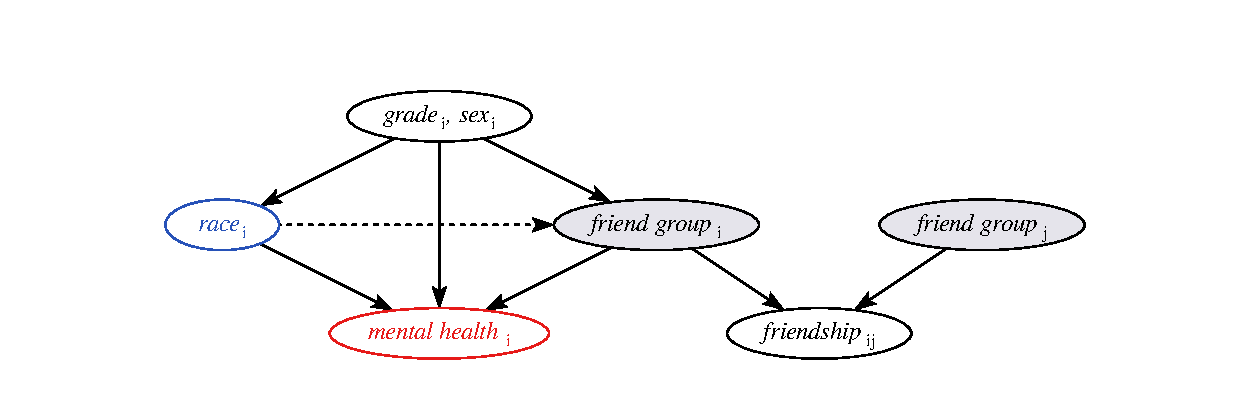
\includegraphics[width=\textwidth]{figures/addhealth-dag.pdf}
        \label{fig:addhealth-dag}
    \end{figure}


\end{frame}

\begin{frame}{Choosing the rank of the network}

    \begin{itemize}
        \item Use cross-validated eigenvalues by \cite{chen_estimating_2021}
        \item Check sensitivity of results to choice of $k$
    \end{itemize}

    \begin{figure}
        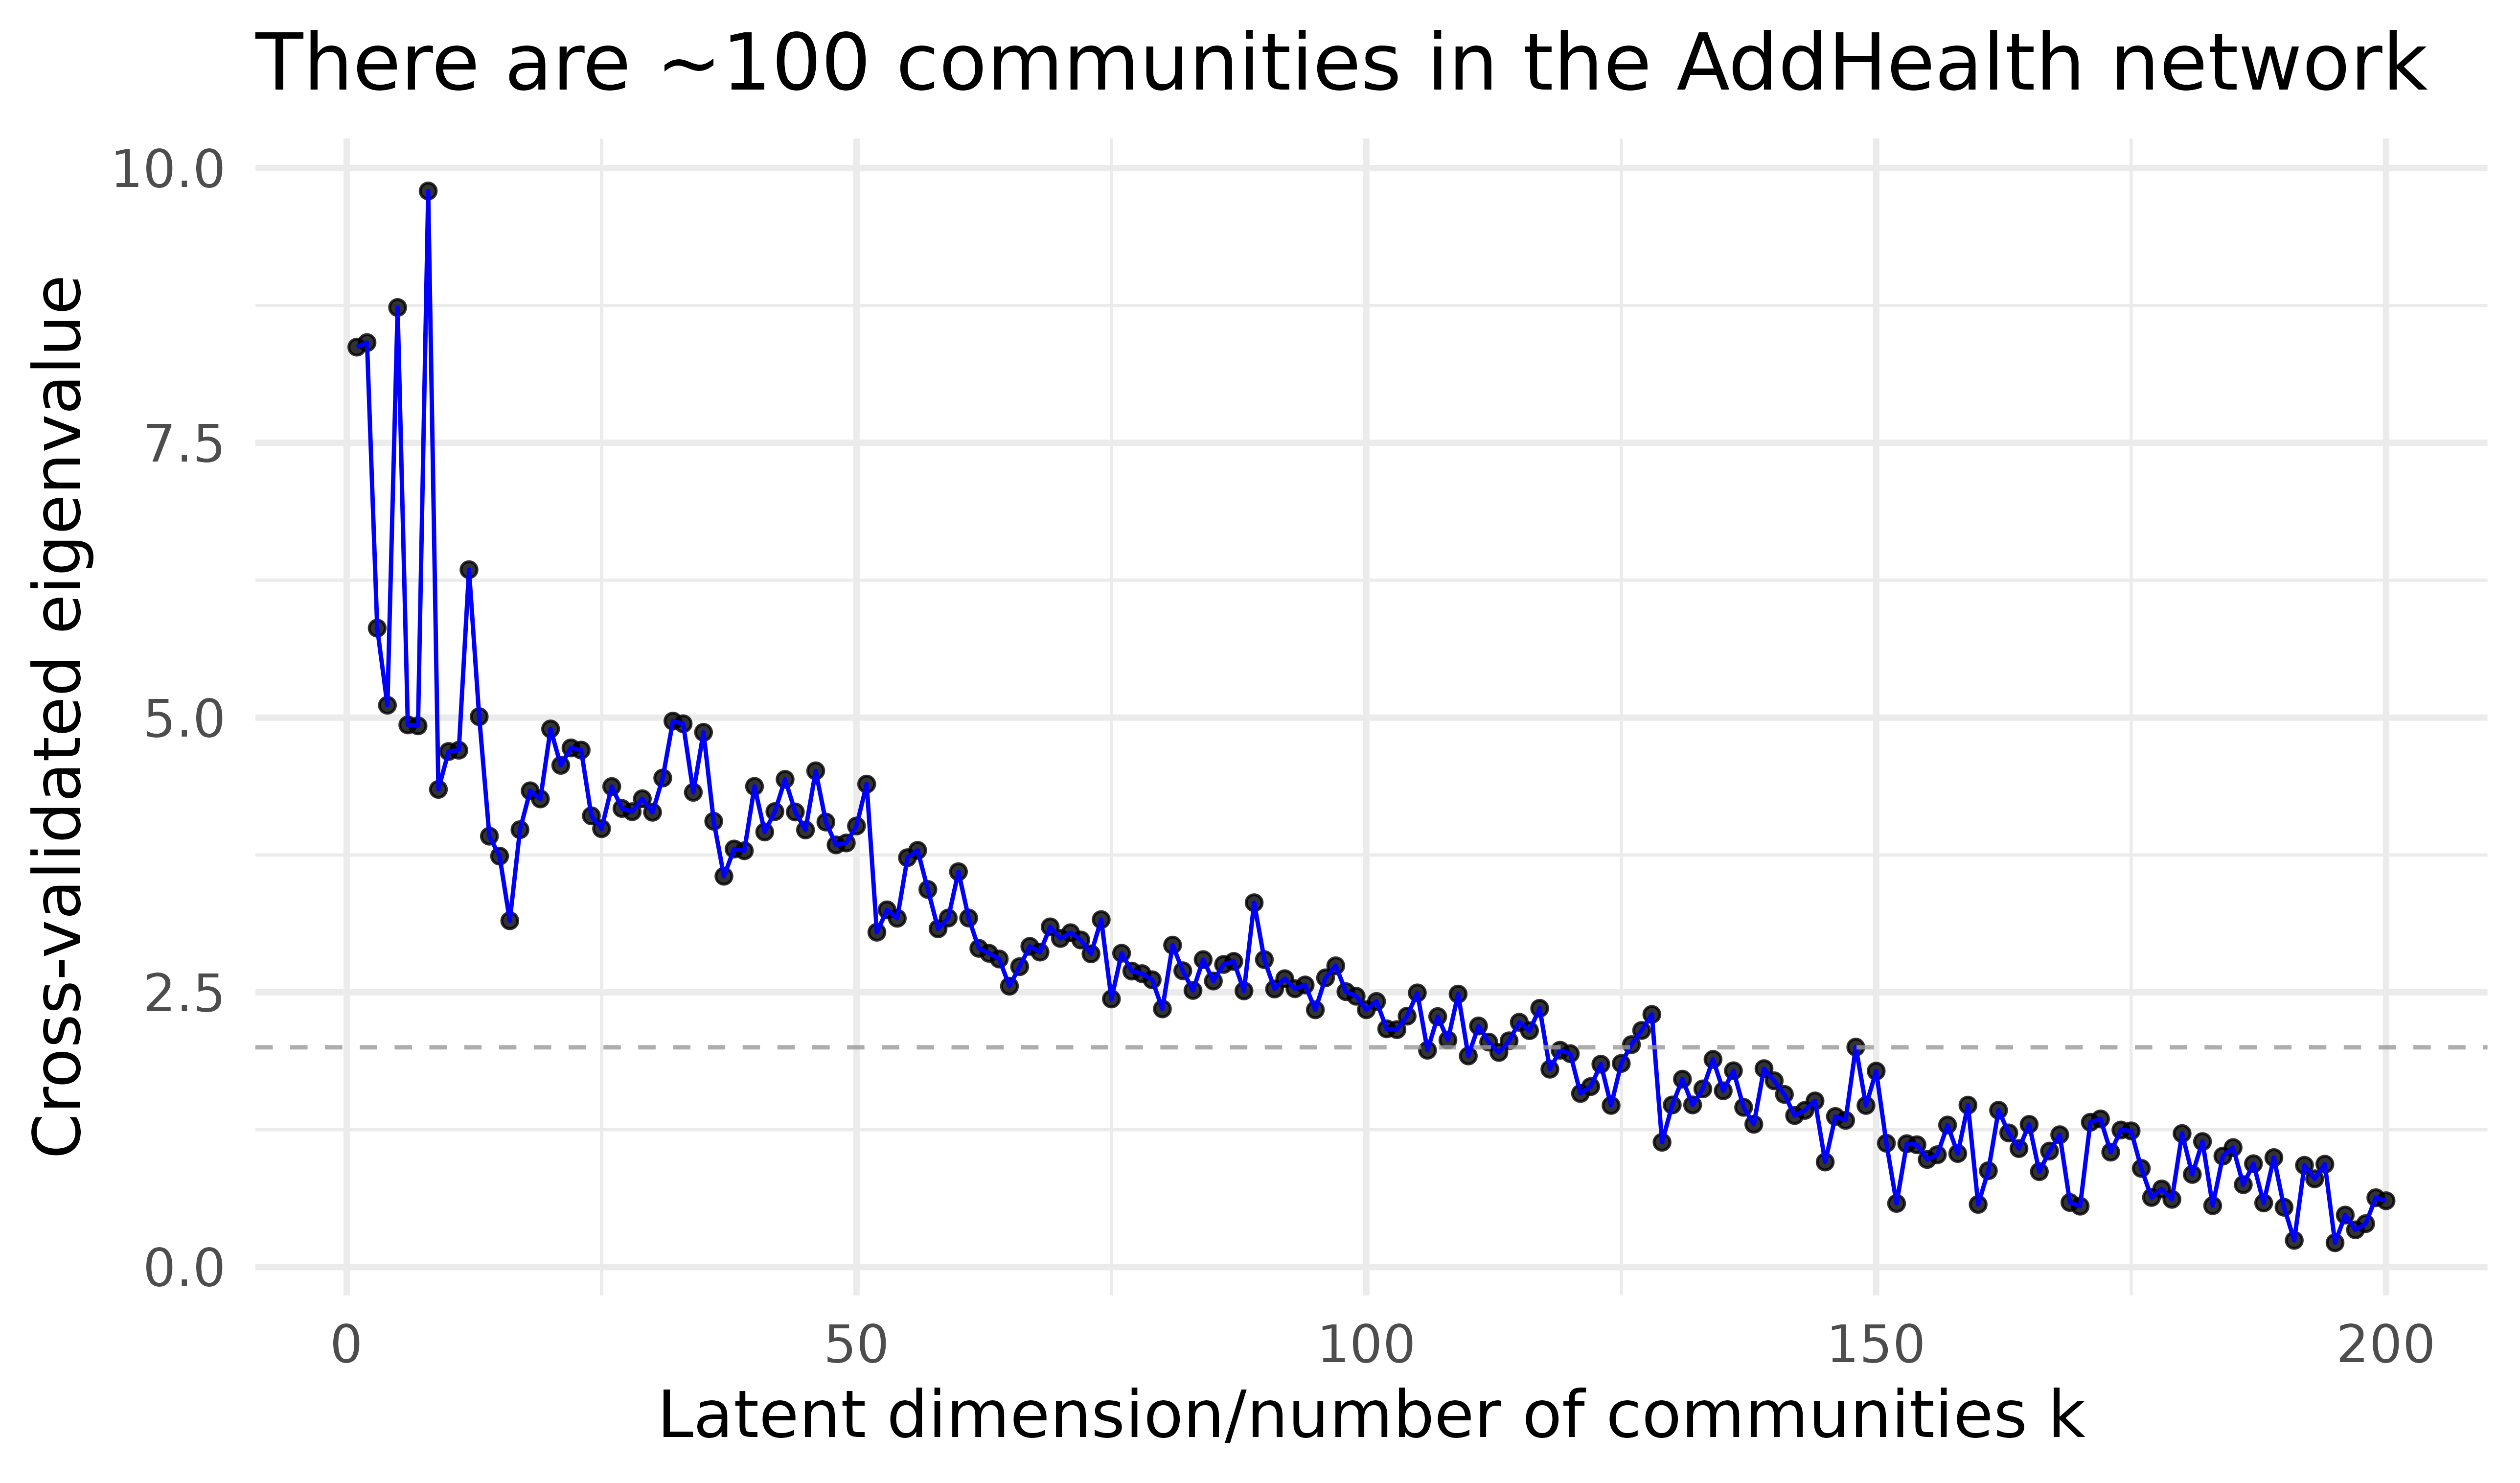
\includegraphics[width=0.9\textwidth]{figures/presentation/rank.png}
        \label{fig:rank}
    \end{figure}

    % Tianxi asks: is the rank estimate too high?
\end{frame}

\begin{frame}{Mediated causal effects in the AddHealth data}

    \begin{figure}
        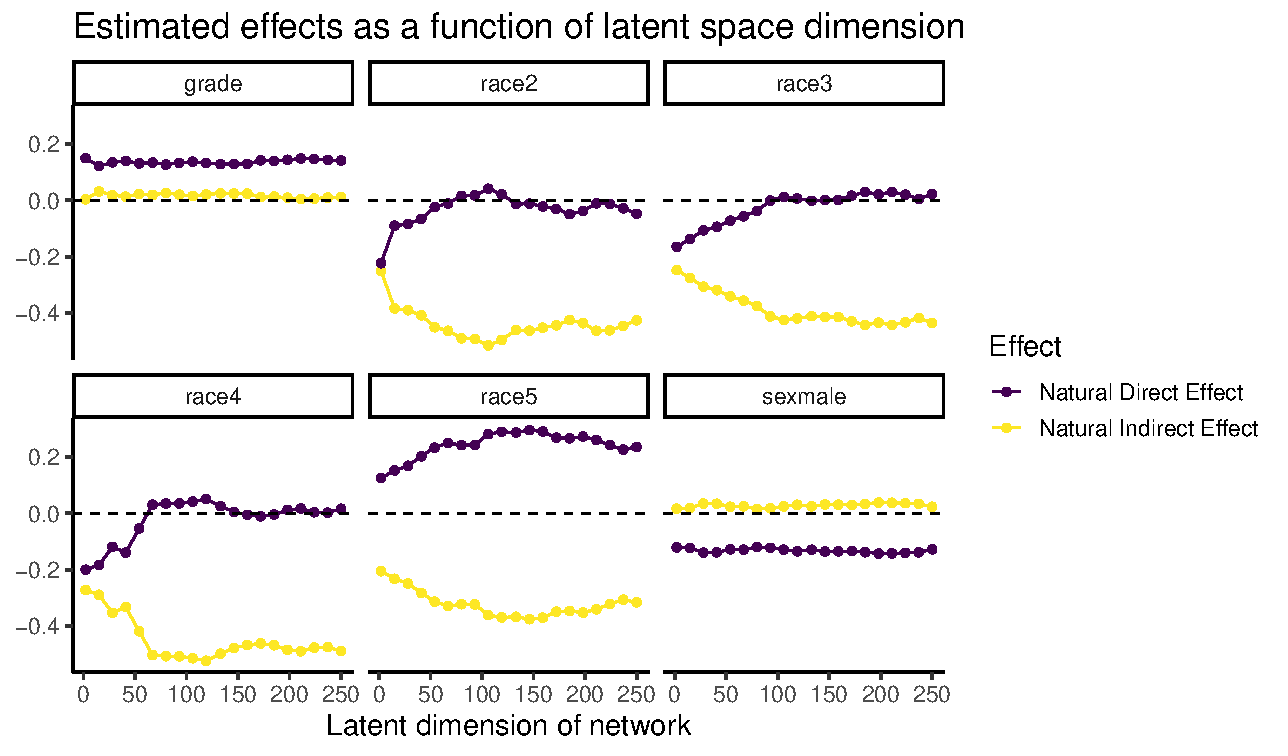
\includegraphics[width=\textwidth]{figures/addhealth-effects.pdf}
        \caption{Point estimates of natural direct and indirect effects in the AddHealth dataset as a function of varying embedding dimension $k$.}
        \label{fig:addhealth-estimates}
    \end{figure}
\end{frame}

\section{Thank you! Questions?}

\begin{frame}{Identifying assumptions as a system of assignments}

    For independent latent $u_{i, \c}, u_{i, t}, u_{i, \x}, u_{i, y}, u_{i, j} \dist \mathrm{Uniform}[0, 1]$ (used for inverse probability transforms), previous DAG equivalent to assuming

    \begin{align*}
        \C_i   & \gets f_C(u_{i, \c})                 \\
        T_i    & \gets f_T(\C_i, u_{i, t})            \\
        \X_i   & \gets f_X(T_i, \C_i, u_{i, \x})      \\
        Y_i    & \gets f_Y(\X_i, T_i, \C_i, u_{i, y}) \\
        A_{ij} & \gets f_A(\X_i, \X_j, u_{i, y})
    \end{align*}

    where $f_C, f_T, f_X, f_Y, f_A$ are arbitrary

\end{frame}

\begin{frame}{Interventions on a network}

    \begin{figure}
        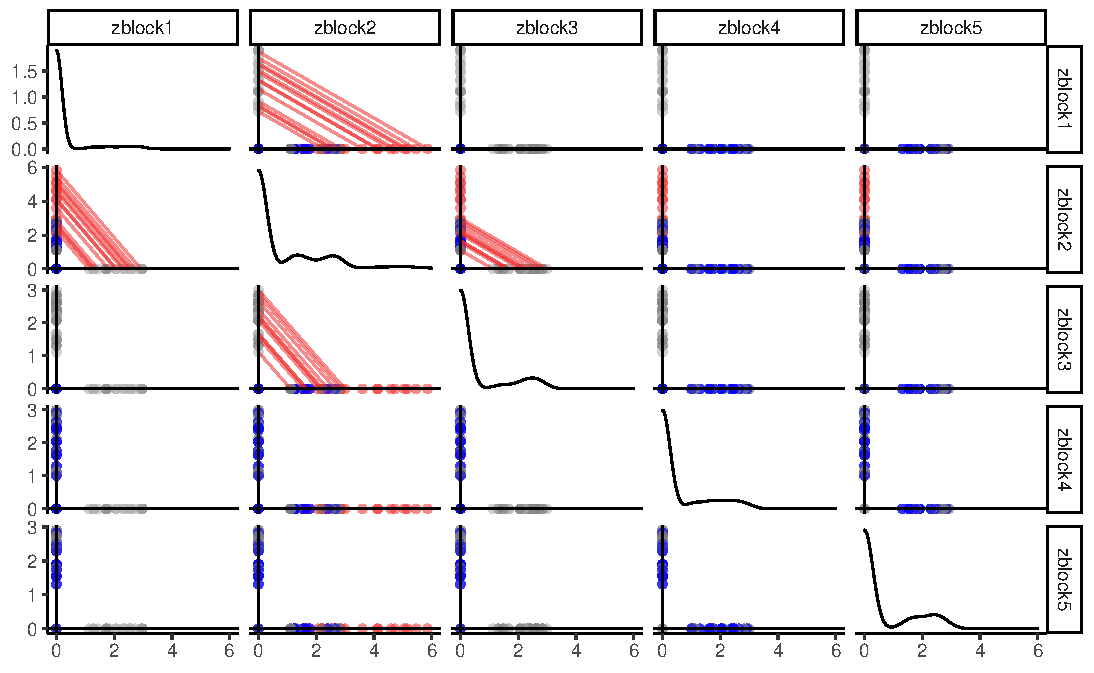
\includegraphics[width=\textwidth]{figures/intervention.pdf}
        \caption{Canonical intervention when $\C$ is highly informative.}
        \label{fig:intervention}
    \end{figure}
\end{frame}

\begin{frame}{Interventions on a network}

    \begin{align*}
        \underbrace{\E[T, \C]{\X}}_{\mathbb R^{1 \times k}}
         & = \underbrace{\thetazero}_{\mathbb R^{1 \times k}}
        + \underbrace{t}_{\{0, 1\}} \underbrace{\thetat}_{\mathbb R^{1 \times k}}
        + \underbrace{\c}_{\mathbb R^{1 \times p}} \underbrace{\Thetac}_{\mathbb R^{p \times k}},
        + \underbrace{t}_{\{0, 1\}} \underbrace{\c}_{\mathbb R^{1 \times p}} \underbrace{\Thetatc}_{\mathbb R^{p \times k}}
    \end{align*}

    In Figure \ref{fig:intervention}, $\C$ are latent parameters for a DC-SBM and $\thetazero = \vec 0, \thetat = \vec 0, \Thetac = I_k$ and

    \begin{align*}
        \Thetatc =
        \begin{bmatrix}
            -1 & 2 & 0  & 0 & 0 \\
            0  & 0 & 0  & 0 & 0 \\
            0  & 1 & -1 & 0 & 0 \\
            0  & 0 & 0  & 0 & 0 \\
            0  & 0 & 0  & 0 & 0 \\
        \end{bmatrix}
    \end{align*}
\end{frame}

\begin{frame}{Abstract}

    The last several years have seen a renewed and concerted effort to incorporate network data into standard tools for regression analysis, and to make network-linked data legible to practicing scientists. Thus far, this literature has primarily developed tools to infer associative relationships between nodal covariates and network structure. In contrast, we augment a statistical model for network regression with counterfactual assumptions and show how causal effects on a network can be partitioned into a direct effect that is uninfluenced by the network, and an indirect effect that is induced by homophily. The method is a conceptually straightforward integration of random dot product models for networks into the well-known product-of-coefficients mediation estimator.

\end{frame}

\bibliographystyle{chicago}
\bibliography{references}

\end{document}